\section{Study 1: variations of facial actions}

This study presents information regarding FA that the subjects presented during the experiment. The 6 hours of recordings of all subjects were manually analyzed and FA were annotated empirically. The annotations were categorized according to the period when they happened (the boring first part or the stressful second part of the games). An analysis on such annotated FA was conducted on group and individual level, aiming to find patterns between the featured FA and the boring/stressful periods of the games.

The following sections presents an analysis, discussion and results of the gathered information.

\subsection{Analysis and methods}

The recordings of all subjects were analyzed by the main author who took notes of any facial actions (FA) that were different from a neutral (resting) face, e.g. lips contraction, brow movement, etc. Annotations were not performed periodically, e.g. every 5 seconds, instead they were made only when the subject's face changed from its neutral/resting state; as a consequence, if the subject remained with a neutral face for a long period of time, no annotations were made during that period.

We decided to use an empirical and non-standard approach for facial annotation as we are not interested in facial expressions \textit{per se}; we want to explore any facial action (standardized or not) that might be used to infer patterns in boredom/stressful states. This approach is not without its limitations, however it provides a reasonable empirical perception of facial activity that is different from a neutral face, which is satisfactory for our investigation. We believe FA are subtle and not necessarily part of a complete facial expression, e.g. surprise face, so they might be better identified in a context where annotations are made only when facial changes happen, as opposed to a frame-by-frame analysis/annotation of a video, for instance.

\begin{figure}[!h]
\centering
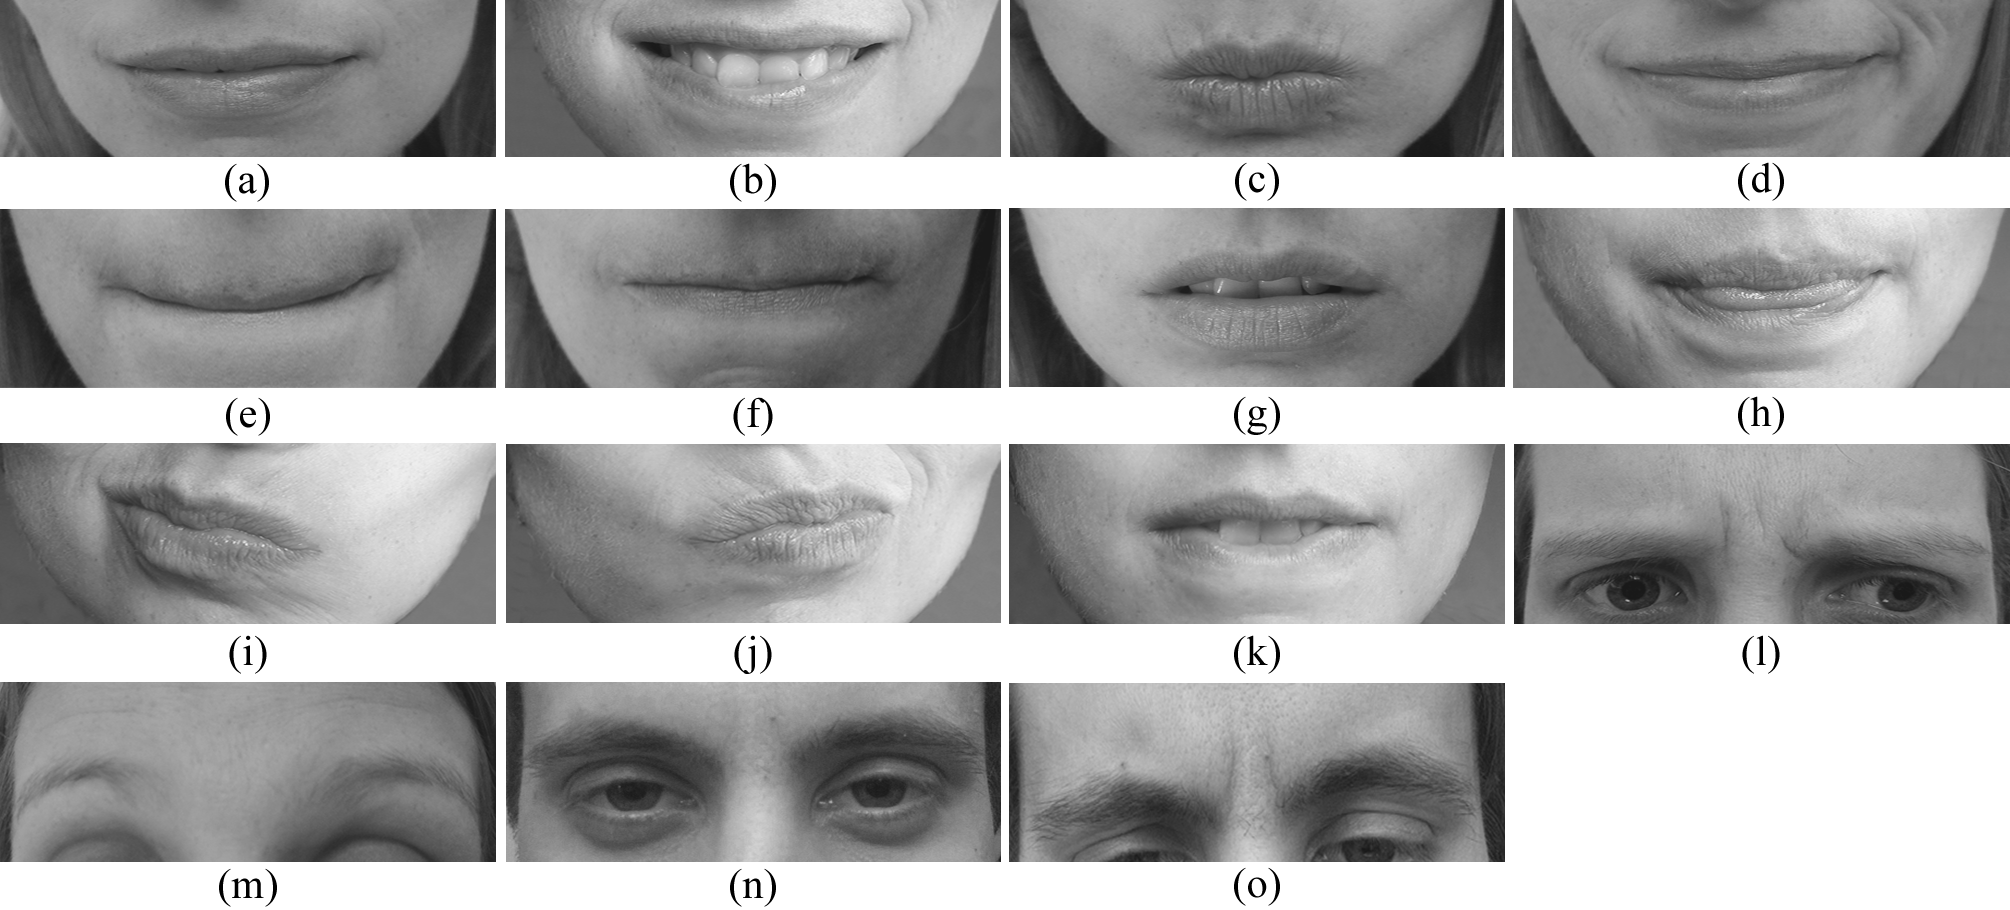
\includegraphics[width=0.4\textwidth]{figures/facial-actions}
\caption{Annotated facial actions (FA). (a) Smile not showing teeth; (b) Smile showing teeth; (c) Lip puckerer; (d) Lip stretcher; (e) Lip suck; (f) Lip pressor; (g) Lips parted; (h) Tongue touching lips; (i) Mouth movement right; (j) Mouth movement left; (k) Lower lip bite; (l) Frown; (m) Brow raiser; (n) Lid tightener; (o) Brow lowering}
\label{fig:fa}
\end{figure}

According to our design of the games, subjects are supposed to perceive the experience during the beginning of the games as being more boring than the one at the end, while the experience at the end should be perceived as more stressing than the one at the beginning of the games. As a result, if we divide in half the game sessions of each subject, in theory one of the two resulting parts is more likely to be perceived as more boring by the subjects, while the other is more likely to be perceived as more stressful. Using that assumption, FA annotations were divided in two groups, the ones made during the period that corresponds to the first half ($H_0$) of the games and the ones made in the second half ($H_1$). Our division of the annotation aimed to identify any pattern regarding FA happening during periods theoretically perceived as boring or stressful. After all annotations were made, we identified which ones were unique and, based on that information, we counted the repetitions of such unique actions across the games for all subjects. As a result, we obtained the frequency that each FA appeared during all game sessions, as well as when they happened (in $H_0$ or $H_1$). We excluded from the list any FA that appeared just a single time during the whole 6 hours recording, assuming that such action was noise or probably part of another action. As a result we identified 17 unique FA that appeared in the recordings at least twice. Excluding the talking and laughing FA, Figure \ref{fig:fa} illustrates all our annotated FA. Finally after all annotations were counted and categorized according to the period in the game, we conducted a per-subject evaluation regarding the frequency of FA. For each subject, we inspected which FA appeared in $H_1$ of all three games with a higher frequency than in $H_0$, and vice versa (appeared in $H_0$ of all three games with a higher frequency than in $H_1$).

\subsection{Results}

\begin{table}[!h]
\renewcommand{\arraystretch}{1.3}
\caption{The amount of FA annotations made for all subjects during the games}
\label{table:amount-fa}
\centering
\begin{tabular}{|c|c|c|}
\cline{2-3}
\multicolumn{1}{c|}{} & \multicolumn{2}{|c|}{\textbf{Period}} \\
\hline
\textbf{Game} & $H_0$ & $H_1$ \\
\hline
Mushroom   & 90 & 98 \\
\hline
Platformer & 88 & 181 \\
\hline
Tetris     & 110 & 159 \\
\hline
\end{tabular}
\end{table}

We analyzed the number of subjects that featured a particular FA, alongside with the number of repetitions of such FA, for all three games. The analysis is also divided according to the period of the game. Only FA featured by two or more subjects were considered, since it produces an analysis that is connected to more frequent FA among the whole group of subjects instead of the peculiarities of a single person. Table \ref{table:amount-fa} shows the amount of FA annotations made for all subjects during the games. According to the results, the amount of FA annotations made during $H_1$ (second half) of all three games was greater than the amount of annotations made during $H_0$ (first half). The increase in annotations during $H_1$ compared to $H_0$ was 8.8\%, 105.6\% and 44.5\% higher for the Mushroom, Platformer and the Tetris game, respectively.

Regarding the FA annotated during each game, for the Mushroom game, the three most frequent FA in $H_0$ were frown (repeated 16 times among 5 subjects), talking (12 times, 3 subjects) and tongue touching lips (9 times, 3 subjects). The three most frequent FA in $H_1$ were frown (repeated 16 times among 3 subjects), talking (13 times, 5 subjects) and lips parted (13 times, 5 subjects). By comparing most frequent FA in the two periods, both frown and talking are present, however they were not featured by a significant number of participants. In fact no more than 5 subjects (25\% of the participants) featured one of those FA. It suggests that individuals present distinct facial behaviors that are not easily generalizable, even in the same context. Curiously, two particular FA presented a significant change in the amount of repetitions and subjects between the two periods: lip pressors (from 7 to 11 repetitions, 2 to 4 subjects) and lips parted (from 5 to 13 repetitions, 2 to 5 subjects). When compared to the whole group of participants, such increase is not significant (again they represent less than 25\% of the participants), but it might be the indication of a pattern for two or three subjects. As suggested by previous work, the combination of such particular changes with another physiological signal, e.g. HR, might produce an acceptable detector for boredom/stress emotional state.

For the Platformer game, the three most frequent FA for $H_0$ were frown (19 repetitions among 3 subjects), tongue touching lips (12 repetitions, 3 subjects) and smile not showing teeth (11 repetitions, 3 subjects). For $H_1$, the FA were frown (49 repetitions, 5 subjects), smile not showing teeth (21 repetitions, 7 subjects) and lips parted (17 repetitions, 5 subjects). By comparing the FA in both periods, frown was featured by more subjects (5, representing 25\%) during the stressful part of the game, however more participants (7, representing 35\%) also featured smiles not showing teeth as well. Additionally to those FA, 25\% of the participants featured talking behavior during $H_1$, externalizing game decisions.

For the Tetris game, the three most frequent FA for $H_0$ were frown (36 repetitions among 4 subjects), smile not showing teeth (14 repetitions, 4 subjects) and lip pressor (11 repetitions, 4 subjects). For $H_1$, the FA were frown (42 repetitions among 4 subjects), lip pressor (28 repetitions, 6 subjects) and smile not showing teeth (16 repetitions, 5 subjects). By comparing those results to the most frequent FA in the Mushroom game, only frown is present in both; it is important to stress that frown was featured by less than 25\% of the participants in both games, which highlights the difficulties in finding a pattern that can be applied to all subjects to identify a boring or a stressful situation, even when the most frequent FA are used. On the other hand, two FA presented a significant change from one period to another in the Tetris game: lip pressor (from 11 to 28 repetitions, 4 to 6 subjects) and talking (from 0 to 15 repetitions, 0 to 6 subjects). Both actions were featured by 30\% of the participants, which could be further investigated in the pursue of FA that can help in the identification of emotional states. Regarding the talking FA, we observed from the recordings that some subjects tended to externalize in words any wrong decisions they made in the game, such as how pieces were positioned, in a similar way observed during the Platformer game; in that sense, talking could be used as an indicator of activity in the game, since it is a clear facial manifestation that happened, in our case, when players were frustrated. For further FA analysis based on a group level, see \parencite{bevilacqua2016variations}.

Finally we conducted a per-subject inspection of all annotated FA according to the procedure described in Section \ref{s:methodology}. We aimed to identify, for each subjects, which FA appeared in $H_0$ (or $H_1$) of \emph{all} three games with a higher frequency than they did in $H_1$ (or $H_0$), if any. Table \ref{table:individual} shows the results of such inspection. Marked numbers represent the frequency of a FA that was present in all three games for the specified subject and period. In total 10 participants (50\%) featured at least one FA that appeared in all three games, in the same period (boring or stressful part) with a frequency equal or greater than its appearance in the counter-period. Subject 2, for instance, featured one lip pressor during $H_0$, while the total number of times the same FA appeared in $H_1$ for all three games combined was 18. We highlight that subject 16 was the only one who featured a FA more frequently in $H_0$ of all three games than he/she did during $H_1$; all other subjects featured FA more frequently in $H_1$ than in $H_0$.

\begin{table}[!h]
\renewcommand{\arraystretch}{1.3}
\caption{Subject-based frequency of FA that appeared in the same period of all three games}
\label{table:individual}
\centering
\begin{threeparttable}
\begin{tabular}{|c|p{4.8cm}|c|c|}
\cline{3-4}
\multicolumn{2}{c|}{} & \multicolumn{2}{|c|}{\textbf{Frequency}} \\
\hline
\textbf{Subject} & \textbf{FA} & \textbf{$H_0$} & \textbf{$H_1$} \\
\hline
2 & Lip pressor & 1 & 18\tnote{b} \\
\hline
15 & Lip pressor & 2 & 9\tnote{b} \\
\hline
10 & Laughing & 2 & 19\tnote{b} \\
\hline
14 & Laughing & 3 & 9\tnote{b} \\
\hline
12 & Smile not showing teeth & 2 & 8\tnote{b} \\
\hline
13 & Smile not showing teeth & 0 & 6\tnote{b} \\
\hline
18 & Smile not showing teeth & 4 & 10\tnote{b} \\
\hline
11 & Lips parted & 1 & 10\tnote{b} \\
\hline
17 & Lip stretcher & 0 & 8\tnote{b} \\
\hline
16 & Talking & 7\tnote{b} & 1 \\
\hline
\end{tabular}
\begin{tablenotes}
\small
\item[b]{FA was present in all three games for the specified subject and period}
\end{tablenotes}
\end{threeparttable}
\end{table}

\subsection{Discussion}

About the FA, even though further investigation is required, our calculations indicate that subjects featured a neutral face for a longer period of time during the first half ($H_0$) of all games when compared to the second half ($H_1$). Since FA annotations were made only when the subject's face featured anything different from her/his neutral face, more annotations indicate more facial activity. Additionally the results might indicate that subjects featured more FA (different from the neutral face) under stressful situations than they did under boring situations, where a neutral face/expression is probably dominant.

Our games were designed to gradually increase the difficulty level until the subject was not able to handle it. As a consequence, we postulate that smiles and laughs during the second half could be connected to the subject's perception that the games were too difficult to continue playing properly. On the other hand, they could indicate genuine manifestations of enjoyment during the moments the subjects felt the game was properly balanced and engaging. Regarding the other FA, such as lip pressor and lips parted, further investigation is required to accurately connect or use such actions to predict/detect emotional states, however the results show a clue about how FA variations can be different on the individual level. As previously discussed, the analysis and generalization of FA on a group level is less clear than an individual approach, since FA behavior might be specific to each person. Our per-subject analysis indicated that, for a portion of the participants, at least one FA was present in the three games, in the same period for the same person. Such information might be used as the starting point for further investigation regarding FA and an individual-tailored detection model for boredom/stress, for instance.

%%%%%%%%%%%%%%%%%%%%%%%%%%%%%%%%%%%%%%%%%%%%%%%%%%%%%%%%%%%%%%%%%%%%%%%%%%%%%%%%%%%%%
%\subsection{Limitations}
%%%%%%%%%%%%%%%%%%%%%%%%%%%%%%%%%%%%%%%%%%%%%%%%%%%%%%%%%%%%%%%%%%%%%%%%%%%%%%%%%%%%%

%One potential limitation of our work is the internal validity. As previously described, the experiment was based on a one-group posttest design, which does not use a control group to measure the effects of the treatment. Such design could be criticized for having low internal validity, since it is not possible to unambiguously attribute cause and effect \parencite{kirk1982experimental}. A two-group approach could be suggested as having stronger internal validity, since it contains a control group and allows a less ambiguous conclusion. In the context of our research, however, any multiple group design implies the comparison of physiological signals and emotional perceptions among different people. Given the social and cultural background of the participants, it is virtually impossible to compare two groups of people regarding stress/boredom. People have different preferences, culture and expectations, which cause maturation and history threats to internal validity \parencite{trochim2001research}. Additionally the process of comparing variations of physiological signals among different subjects is a complex task, even when subjects are similar, e.g. same age and sex. As a consequence, a subject in a control group might present a set of variations of signals and classify a game as boring, while a similar subject in another group might classify the same game as not boring at all, presenting a different set of variations of signals. In that light, our experiment relies on a one-group experimental design to increase internal validity, since subjects were compared with themselves, which removes inter-subject differences.

%Another limitation is the empirical approach used to annotate the FA, which was not based on a formal scheme and was conducted by a single person without validation by other researchers. We believe that the exploratory nature of our study regarding FA allows the use of such approach. Our aim was not to standardize FA regarding stress/boredom, but to document the perceptions of naked-eye observations of FA in a context involving games, so that it can be used to guide further steps regarding the utilization of FA in a multifactorial analysis. A frame-by-frame annotation of our video recordings using a formal scheme, such as FACS, would be a significantly laborious and time-consuming task, which is not motivated by our exploratory and empirical approach. Another limitation is the assumption used when dividing each game session in half, presuming that the middle point of the period indicates a transition from two distinct periods: $H_0$, perceived as more boring, and $H_1$, perceived as more stressing. It is not necessarily true. Even though our data indicate that subjects perceived the beginning of the games as being boring and the end as being stressful, our point of division or the periods themselves remain an assumption. There might be moments towards the end of the game, for instance, that could be perceived as more boring or joyful depending on the subject, since each participant has her/his own specific expectations and skill level regarding games. Finally the core mechanic of the Mushroom game is based on the color of the mushrooms (instead of patterns, for instance), which is not suitable for color blind subjects.

\subsection{Conclusion}

%This paper presented the description and results of an experiment aimed at exploring the variations of heart rate (HR) and facial actions (FA) during gaming sessions with induced boredom and stress. In total twenty adults of different ages and gaming experiences participated in the experiment, where they played three different games while being recorded by a video camera and monitored by a HR sensor. The games used in the experiment were carefully designed and implemented to have a difficulty level that linearly increases over time, from a boring to a stressful point. According to self-reported answers in post-games questionnaires, participants perceived the games as being boring at the beginning and stressful at the end. Such configuration gives our experiment a novel approach for the exploration of HR and FA regarding their connection to emotional states, since information can be categorized according to the induced (and theoretically known) emotional states.

Results show that more FA annotations were made during the stressful part of the games, which indicates that participants remained with a neutral face for longer periods of time during the boring part. The analysis on group level revealed that any FA pattern was related to 5 subjects (25\% of the group) at most. In the analysis conducted on the individual level, particular patterns were found for 10 subjects (50\% of the group).

%Our findings suggest that changes in the HR during gaming sessions is a promising indicator of stress, which could be incorporated into a model aimed at emotion detection. As pointed out by previous work, a user-tailored model based on several signals, e.g. HR and FA, is more likely to detect emotional states of users. In the context where the measurement of physiological signals by physical and contact-based sensors is intrusive or not desired, e.g. remote estimation of HR, information from different channels is required. One of such additional channels of information might be facial expressions, such as the FA analysis performed in this paper. For the context of our experiment, FA analysis on an individual level produced more information to connect FA and stress/boredom emotional states. We believe that this paper contributes with information regarding HR and FA in the context of games, which can be combined to create user-tailored models for emotion detection based on different data sources.
